\chapter{Objectives Specification and Work Environment}

\section*{Introduction}
This chapter will first define the project's functional and non-functional requirements, then we will discuss the chosen cryptographic algorithms, explaining the reasoning behind their selection and offering an overview of how each algorithm works. Finally we will specify the hardware and software resources necessary for this demonstration. 

\section{Project Specification}
Requirements analysis is a fundamental phase in every project realization process. It is based on the study of the project's features as well as the constraints. In this section, we will cover both the functional and non-functional requirements.

\subsection{Functional Requirements}

The goal of the "CryptoEngine" demo is to establish secure communication between an STM32XX MCU using "CryptoEngine" and an STM32U5 MCU using PKA and AES. Secure communication means guaranteeing the three key security concepts: confidentiality, integrity, and authenticity.

\begin{itemize}
    \item \textbf{Confidentiality:} Ensuring that only authorized parties can understand the messages exchanged. This is achieved through:
    \begin{itemize}
        \item \textbf{Asymmetric Key Management:} Implement asymmetric key  management for ECDSA and ECDH keys, ensuring secure storage and handling of private keys and generation of public keys.
        \item \textbf{Shared Secret Computation:} Compute the ECDH shared secret using the exchanged public keys, which will be used as the basis for deriving symmetric encryption keys.
    \end{itemize}
    
    \item \textbf{Integrity:} Ensuring that the message has not been altered during transmission. This is achieved through:
    \begin{itemize}
       \item \textbf{Symmetric Message Encryption and Decryption:} Use AES GCM symmetric encryption to encrypt messages and verify their integrity during transmission. This also serves as an authentication check.
    \end{itemize}
    
    \item \textbf{Authenticity:} Ensuring that the communicating parties are who they claim to be. This is achieved through:
    \begin{itemize}
        \item \textbf{Signature Generation and Verification:} Enable the generation and verification of digital signatures using ECDSA to ensure the authenticity of the communicating parties.
    \end{itemize}
\end{itemize}

Establishing a secure, authenticated encryption system using modern cryptographic standards, including Elliptic Curve Digital Signature Algorithm (ECDSA) for digital signatures, Elliptic Curve Diffie-Hellman (ECDH) for key exchange, and Advanced Encryption Standard Galois Counter Mode (AES GCM) for encryption and authentication, is the primary goal.

Table \ref{tab:functional_requirements} neatly summarizes the functional requirements for our demonstration.

\setlength{\tabcolsep}{10pt} % Adjust the padding
\renewcommand{\arraystretch}{1.5} % Adjust the row height

\begin{table}[h]
\centering
\caption{Functional Requirements for Secure Communication}
\label{tab:functional_requirements}
\begin{tabular}{|m{2.5cm}|p{3.5cm}|p{9cm}|}
\hline
\textbf{Security Requirement} & \textbf{Component} & \textbf{Description} \\ \hline
\multirow{2}{*}{Confidentiality} & Key Management & Implement key management for ECDSA and ECDH keys, ensuring
secure storage and handling of private keys and generation of public keys. \\ \cline{2-3} 
 & Shared Secret Computation & Compute the ECDH shared secret using the exchanged public keys, which will be used as the basis for deriving symmetric encryption keys. \\ \hline
Integrity & Message Encryption and Decryption & Use AES GCM to encrypt messages and verify their integrity during transmission. This also serves as an additional authenticity verification. \\ \hline
Authenticity & Signature Generation and Verification & Enable the generation and verification of digital signatures using ECDSA to ensure the authenticity of the communicating parties. \\ \hline
\end{tabular}
\end{table}

\subsection{Non-Functional Requirements}
Below are the non-functional requirements or the constraints that the functional expectations must abide by:
\begin{itemize}
    \item \textbf{Clarity:} The demo should be clear and easily understandable, enabling users without extensive technical expertise to grasp the concepts.
     \item \textbf{Transferability:} The knowledge and experience gained from the demo should empower users to apply cryptographic techniques in their own projects with ease.
   \item \textbf{Modularity:} The demo should be designed in a modular way, allowing individual components to be easily reused or adapted for different applications.
  \item \textbf{Feature Comparison:} The demo should highlight the new features and enhancements introduced by the "CryptoEngine" compared to its predecessors, demonstrating the improvements in security and usability.
\end{itemize}

\section{Cryptographic Decisions and Context}
Before delving further into the implementation details, it is crucial to understand the rationale behind the cryptographic algorithms and protocols chosen for this demo. This section elucidates the reasons for selecting specific cryptographic methods and their relevance to the project's objectives.

\subsection{Elliptic Curve Diffie-Hellman}
Elliptic Curve Diffie-Hellman (ECDH) is a widely adopted key exchange protocol that facilitates secure and efficient key exchange between parties. We opted for ECDH due to its significant advantages over traditional algorithms like RSA, particularly in resource-constrained environments.

\begin{itemize}
    \item \textbf{Resource Efficiency:} ECDH is less resource-intensive compared to RSA, making it suitable for embedded systems with limited computational power and memory.
     \item \textbf{Optimal Key Size:} A 256-bit key size strikes a balance between security and performance, making it suitable for embedded applications, including our demo.
    
\end{itemize}

\begin{figure}[H]
    \centering
    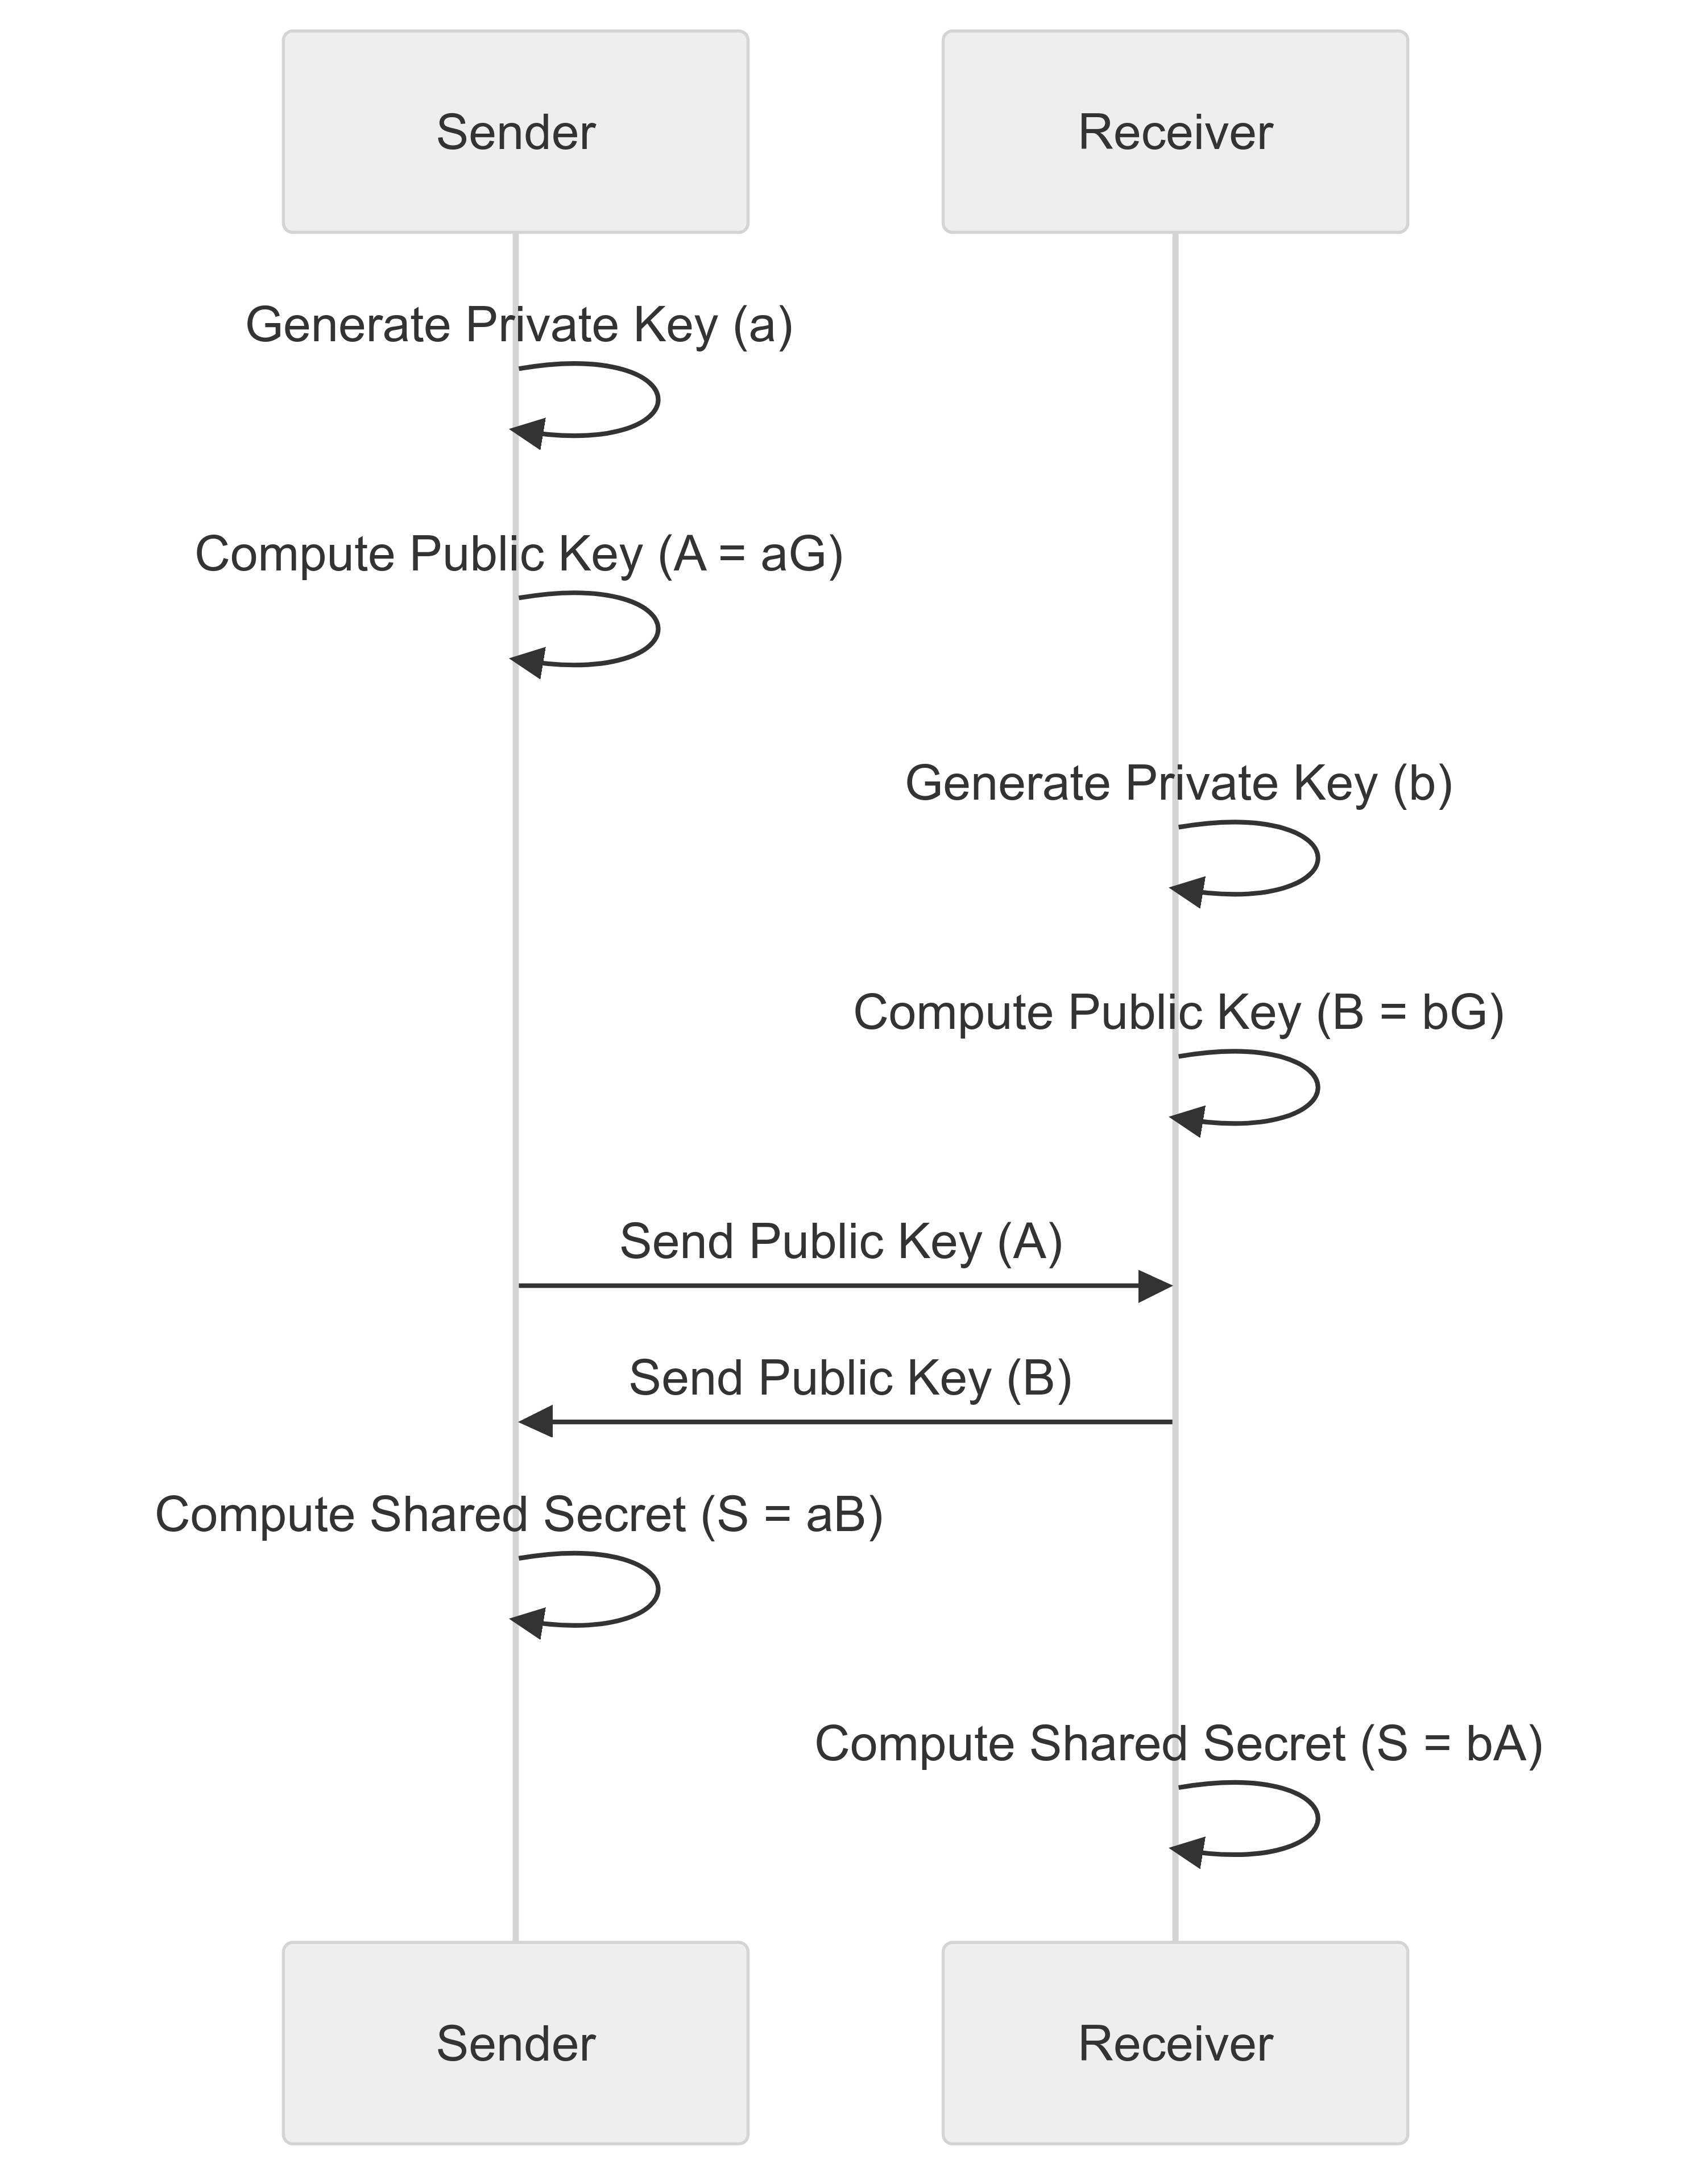
\includegraphics[width=10cm]{img/ECDH.png}
    \caption{Elliptic Curve Diffie Hellman Process}
    \label{fig:ecdh_graph}
\end{figure} 

The ECDH process as shown in Figure \ref{fig:ecdh_graph}, begins with both the sender and the receiver independently generating their own private and public key pairs.

The sender generates a private key \(a\) and computes their corresponding public key \(A = aG\), where \(G\) is a predefined generator point on the elliptic curve. Similarly, the receiver generates a private key \(b\) and computes their corresponding public key \(B = bG\).

Once the key pairs are generated, the sender and receiver exchange their public keys over the insecure channel. The sender sends their public key \(A\) to the receiver, and the receiver sends their public key \(B\) to the sender. Despite the exchange occurring over an insecure channel, the private keys \(a\) and \(b\) remain confidential and are never transmitted.

After receiving the public key from the other party, each participant computes the shared secret using their own private key and the received public key. The sender calculates the shared secret \(S = aB\) by multiplying their private key \(a\) with the receiver's public key \(B\). Conversely, the receiver calculates the shared secret \(S = bA\) by multiplying their private key \(b\) with the sender's public key \(A\). Due to the properties of elliptic curves, both computations result in the same shared secret \(S\), which can be used to derive a symmetric key for encrypting and decrypting subsequent communications.



\subsection{Elliptic Curve Digital Signature Algorithm}
The Elliptic Curve Digital Signature Algorithm (ECDSA) is a renowned digital signature algorithm that enables the generation and verification of digital signatures, ensuring data authenticity and integrity.

\begin{itemize}
    \item \textbf{Efficiency:} ECDSA is highly efficient, offering faster computations and smaller key sizes compared to other digital signature algorithms like RSA.
    \item \textbf{Compatibility:} ECDSA is supported by the PKA (Public Key Accelerator) peripheral in STM32 products, making it an ideal choice for our demo.
    \item \textbf{Security:} ECDSA provides strong security guarantees, leveraging the hardness of the elliptic curve discrete logarithm problem.
\end{itemize}

The graph in Figure \ref{fig:ecdsa_graph} illustrates a typical digital signature process that applies to many algorithms, including ECDSA. It involves two main phases: signing by the sender and verification by the receiver. 

On the sender side, the process begins with key generation, where a pair of keys—a private key and a public key—are created. The sender then prepares a message that needs to be signed. This message is passed through a hashing algorithm to produce a message hash, ensuring that the message is represented in a fixed-size format. The private key and the message hash are then input into the signing algorithm to generate a signature. Subsequently, the message, signature, and public key are transmitted to the receiver.

On the receiver side, the verification algorithm uses the public key, message hash, and signature to verify the authenticity of the message. The receiver independently generates the message hash using the same hashing algorithm as the sender. If the signature is valid, the sender is authenticated, providing confidence that the message has not been tampered with and is from the legitimate sender. Conversely, if the signature is invalid, the sender is not authenticated, indicating potential tampering or an illegitimate sender. This process ensures both the integrity and authenticity of the message, making digital signatures a necessity for secure communications.

\begin{figure}[H]
    \centering
    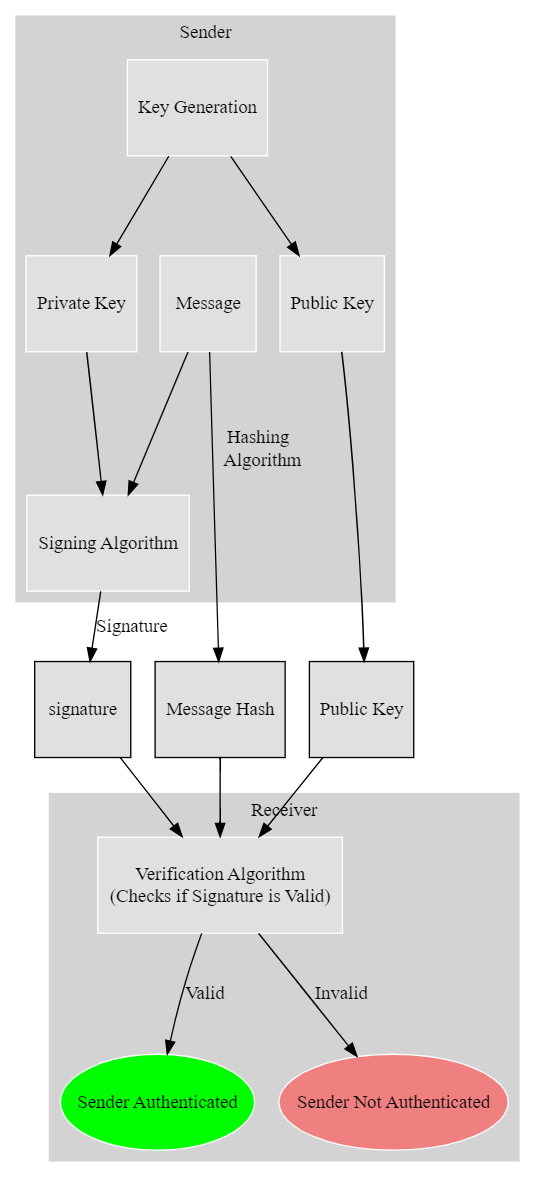
\includegraphics[width=7.5cm]{img/TD ECDSA Graph.png}
    \caption{Typical Digital Signature Process}
    \label{fig:ecdsa_graph}
\end{figure}


\subsection{NIST P-256 Curve}
\label{curve_param}
For this demo, we have chosen the NIST P-256 curve for both the ECDSA algorithm and the ECDH protocol. This decision was based on several factors:

\begin{itemize}
    \item \textbf{NIST Recommendation:} The P-256 curve is recommended by the National Institute of Standards and Technology (NIST) for its security and efficiency \cite{nist_p256}.
    \item \textbf{Popularity:} The P-256 curve is widely used and well-supported across various cryptographic libraries and tools, facilitating interoperability and ease of use \cite{Telemetry}.
    \item \textbf{Documentation:} Extensive documentation and implementation examples are available for the P-256 curve, simplifying the development and debugging processes.
    \item \textbf{Smaller Key Size:} ECDH achieves the same security level as RSA with much smaller key sizes. For instance, a 256-bit key in ECDH provides equivalent security to a 3072-bit key in RSA, as illustrated in Table \ref{tab:rsa_vs_ecc}.
   
    
\end{itemize}
\begin{table}[H]
    \caption{Comparison of Key Sizes and Security Levels between RSA and ECC}
    \centering
    \begin{tabular}{|c|c|c|}
        \hline
        \textbf{Algorithm} & \textbf{Key Size (bits)} & \textbf{Security Level (bits)} \\
        \hline
      
        RSA & 2048 & 112 \\
        \hline
        RSA & 3072 & 128 \\
        \hline
        RSA & 15360 & 256 \\
        \hline
        ECC (P-224) & 224 & 112 \\
        \hline
        ECC (P-256) & 256 & 128 \\
        \hline
        ECC (P-521) & 521 & 256 \\
        \hline
    \end{tabular}

    \label{tab:rsa_vs_ecc}
\end{table}
\textit{Note: Using a 256-bit curve means that private keys will be 256 bits long, and our public key's x and y coordinates will each be 256 bits long, totaling 512-bit size for the public keys.}


\subsection{AES Galois Counter Mode}
AES Galois Counter Mode (GCM) is a robust symmetric encryption algorithm that provides both confidentiality and integrity. We chose AES GCM for the following reasons:

\begin{itemize}
    \item \textbf{High Security:} AES GCM offers strong security guarantees, making it resistant to various cryptographic attacks. It is widely regarded as one of the most secure modes of operation for AES.
    \item \textbf{Integrity and Authenticity:} AES GCM generates an authentication tag during encryption, which can be used to verify the integrity and authenticity of the encrypted data. This dual functionality is particularly valuable in ensuring data security.
    \item \textbf{Standardization:} AES GCM is a standardized encryption mode, widely adopted in various security protocols and applications, ensuring compatibility and interoperability.
\end{itemize}
Figure \ref{fig:aes_gcm} \cite{U5_Refman} illustrates the AES GCM process.
It begins with the initialization vector being fed into a counter. The counter's value, along with the symmetric encryption key, is used by the AES encryption function to generate a series of encrypted blocks. These encrypted blocks are then XORed with the corresponding plaintext blocks to produce the ciphertext.

Simultaneously, the encrypted blocks are processed through a Galois field multiplication (GF2mul), which contributes to generating an authentication tag (TAG) for integrity verification. The output of the AES GCM process is both the encrypted message (ciphertext) and the authentication tag, ensuring confidentiality and integrity of the data. The diagram also shows the handling of additional blocks and the finalization step to complete the authentication process.

\begin{figure}[H]
  \centering
  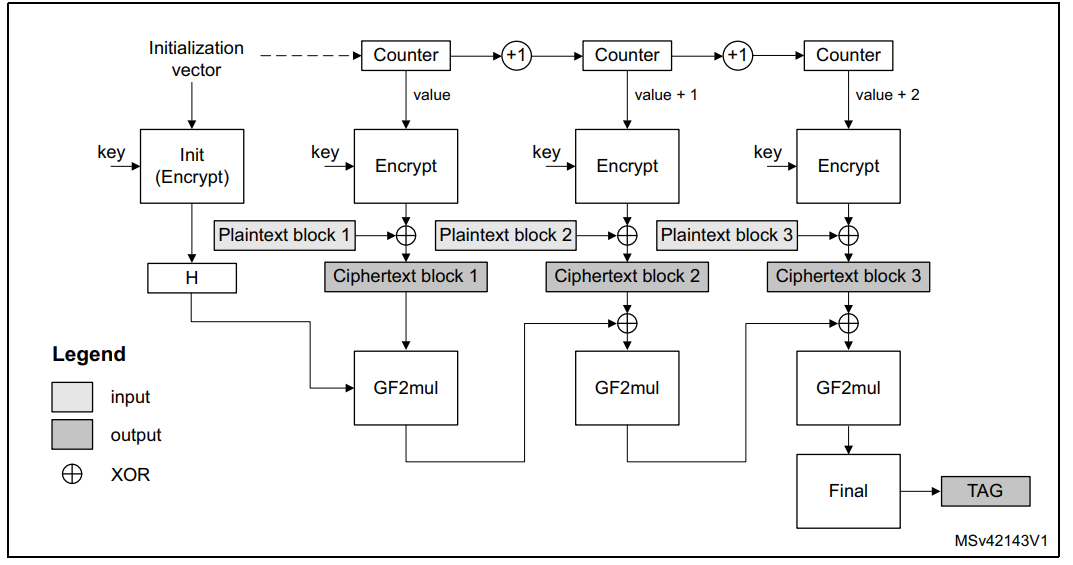
\includegraphics[width=17cm]{img/AES GCM.png}
  \caption{AES Galois Counter Mode Process }
  \label{fig:aes_gcm}
\end{figure}

\section{Use-Case Diagram}
\begin{figure}[H]
  \centering
  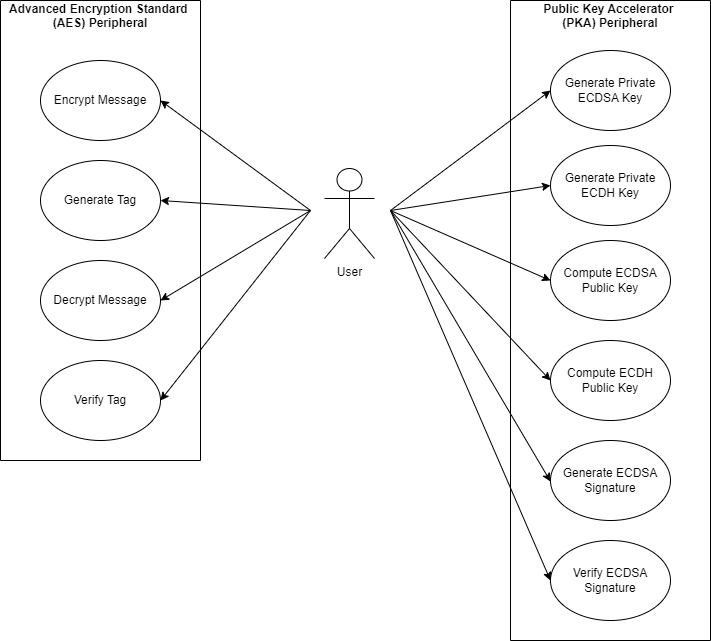
\includegraphics[width=14.5cm]{img/use case 2.png}
  \caption{Use-Case Diagram for Cryptographic Peripherals (AES and PKA)}
  \label{fig:use_case_diagram}
\end{figure}

The Use-Case diagram in Figure \ref{fig:use_case_diagram} illustrates the interactions between a user and the cryptographic peripherals available on STM32 MCUs.
 Refer to Table \ref{tab:use_cases} for an in-depth explanation:

\begin{longtable}{|p{5cm}|p{6cm}|p{4cm}|}
\caption{Use Cases for Cryptographic Peripherals} \label{tab:use_cases} \\

\hline
\textbf{Use Case} & \textbf{Relevance} & \textbf{Peripheral Used} \\ \hline
\endfirsthead

\multicolumn{3}{c}%
{{\bfseries \tablename\ \thetable{} -- continued from previous page}} \\
\hline
\textbf{Use Case} & \textbf{Relevance} & \textbf{Peripheral Used} \\ \hline
\endhead

\hline \multicolumn{3}{|r|}{{Continued on next page}} \\ \hline
\endfoot

\hline
\endlastfoot

Generate Private ECDSA Key & Part of the key management process, ensuring secure storage and handling of private keys, which contributes to confidentiality. & PKA (Public Key Accelerator) \\ \hline
Generate Private ECDH Key & Part of the key management process and essential for establishing a shared secret, contributing to confidentiality. & PKA (Public Key Accelerator) \\ \hline
Compute ECDSA Public Key & Necessary for signature verification, which ensures authenticity. & PKA (Public Key Accelerator) \\ \hline
Compute ECDH Public Key & Necessary for the ECDH key exchange process, contributing to confidentiality. & PKA (Public Key Accelerator) \\ \hline
Generate ECDSA Signature & Ensures the authenticity of the communicating parties by providing a way to verify identities. & PKA (Public Key Accelerator) \\ \hline
Verify ECDSA Signature & Ensures the authenticity of the communicating parties by verifying the provided signatures. & PKA (Public Key Accelerator) \\ \hline
Encrypt Message & Ensures confidentiality and integrity of the message during transmission. & AES (Advanced Encryption Standard) \\ \hline
Generate Tag & Ensures the integrity of the message and also serves as an authentication check. & AES (Advanced Encryption Standard) \\ \hline
Decrypt Message & Ensures confidentiality and integrity of the message during transmission. & AES (Advanced Encryption Standard) \\ \hline
Verify Tag & Ensures the integrity of the message and also serves as an authentication check. & AES (Advanced Encryption Standard) \\ \hline

\end{longtable}






\section{Work Environment}
In this section, we outline the hardware and software resources utilized during the internship project that were essential for the development, testing, and demonstration of the "CryptoEngine" peripheral.

\subsection{Hardware Resources}
\begin{itemize}
    \item \textbf{STM32XX MCU:} The STM32XX microcontroller unit (MCU) is the primary hardware platform used for implementing and testing the "CryptoEngine" peripheral. The STM32XX series offers advanced cryptographic features and peripherals, making it ideal for secure communication applications.
    \item \textbf{STM32U545 MCU:} The STM32U545 microcontroller unit is used for comparison and interoperability with the STM32XX MCU. This board utilizes the AES and PKA peripherals to perform cryptographic operations, enabling secure key exchange and encryption.
    \begin{figure}[H]
  \centering
  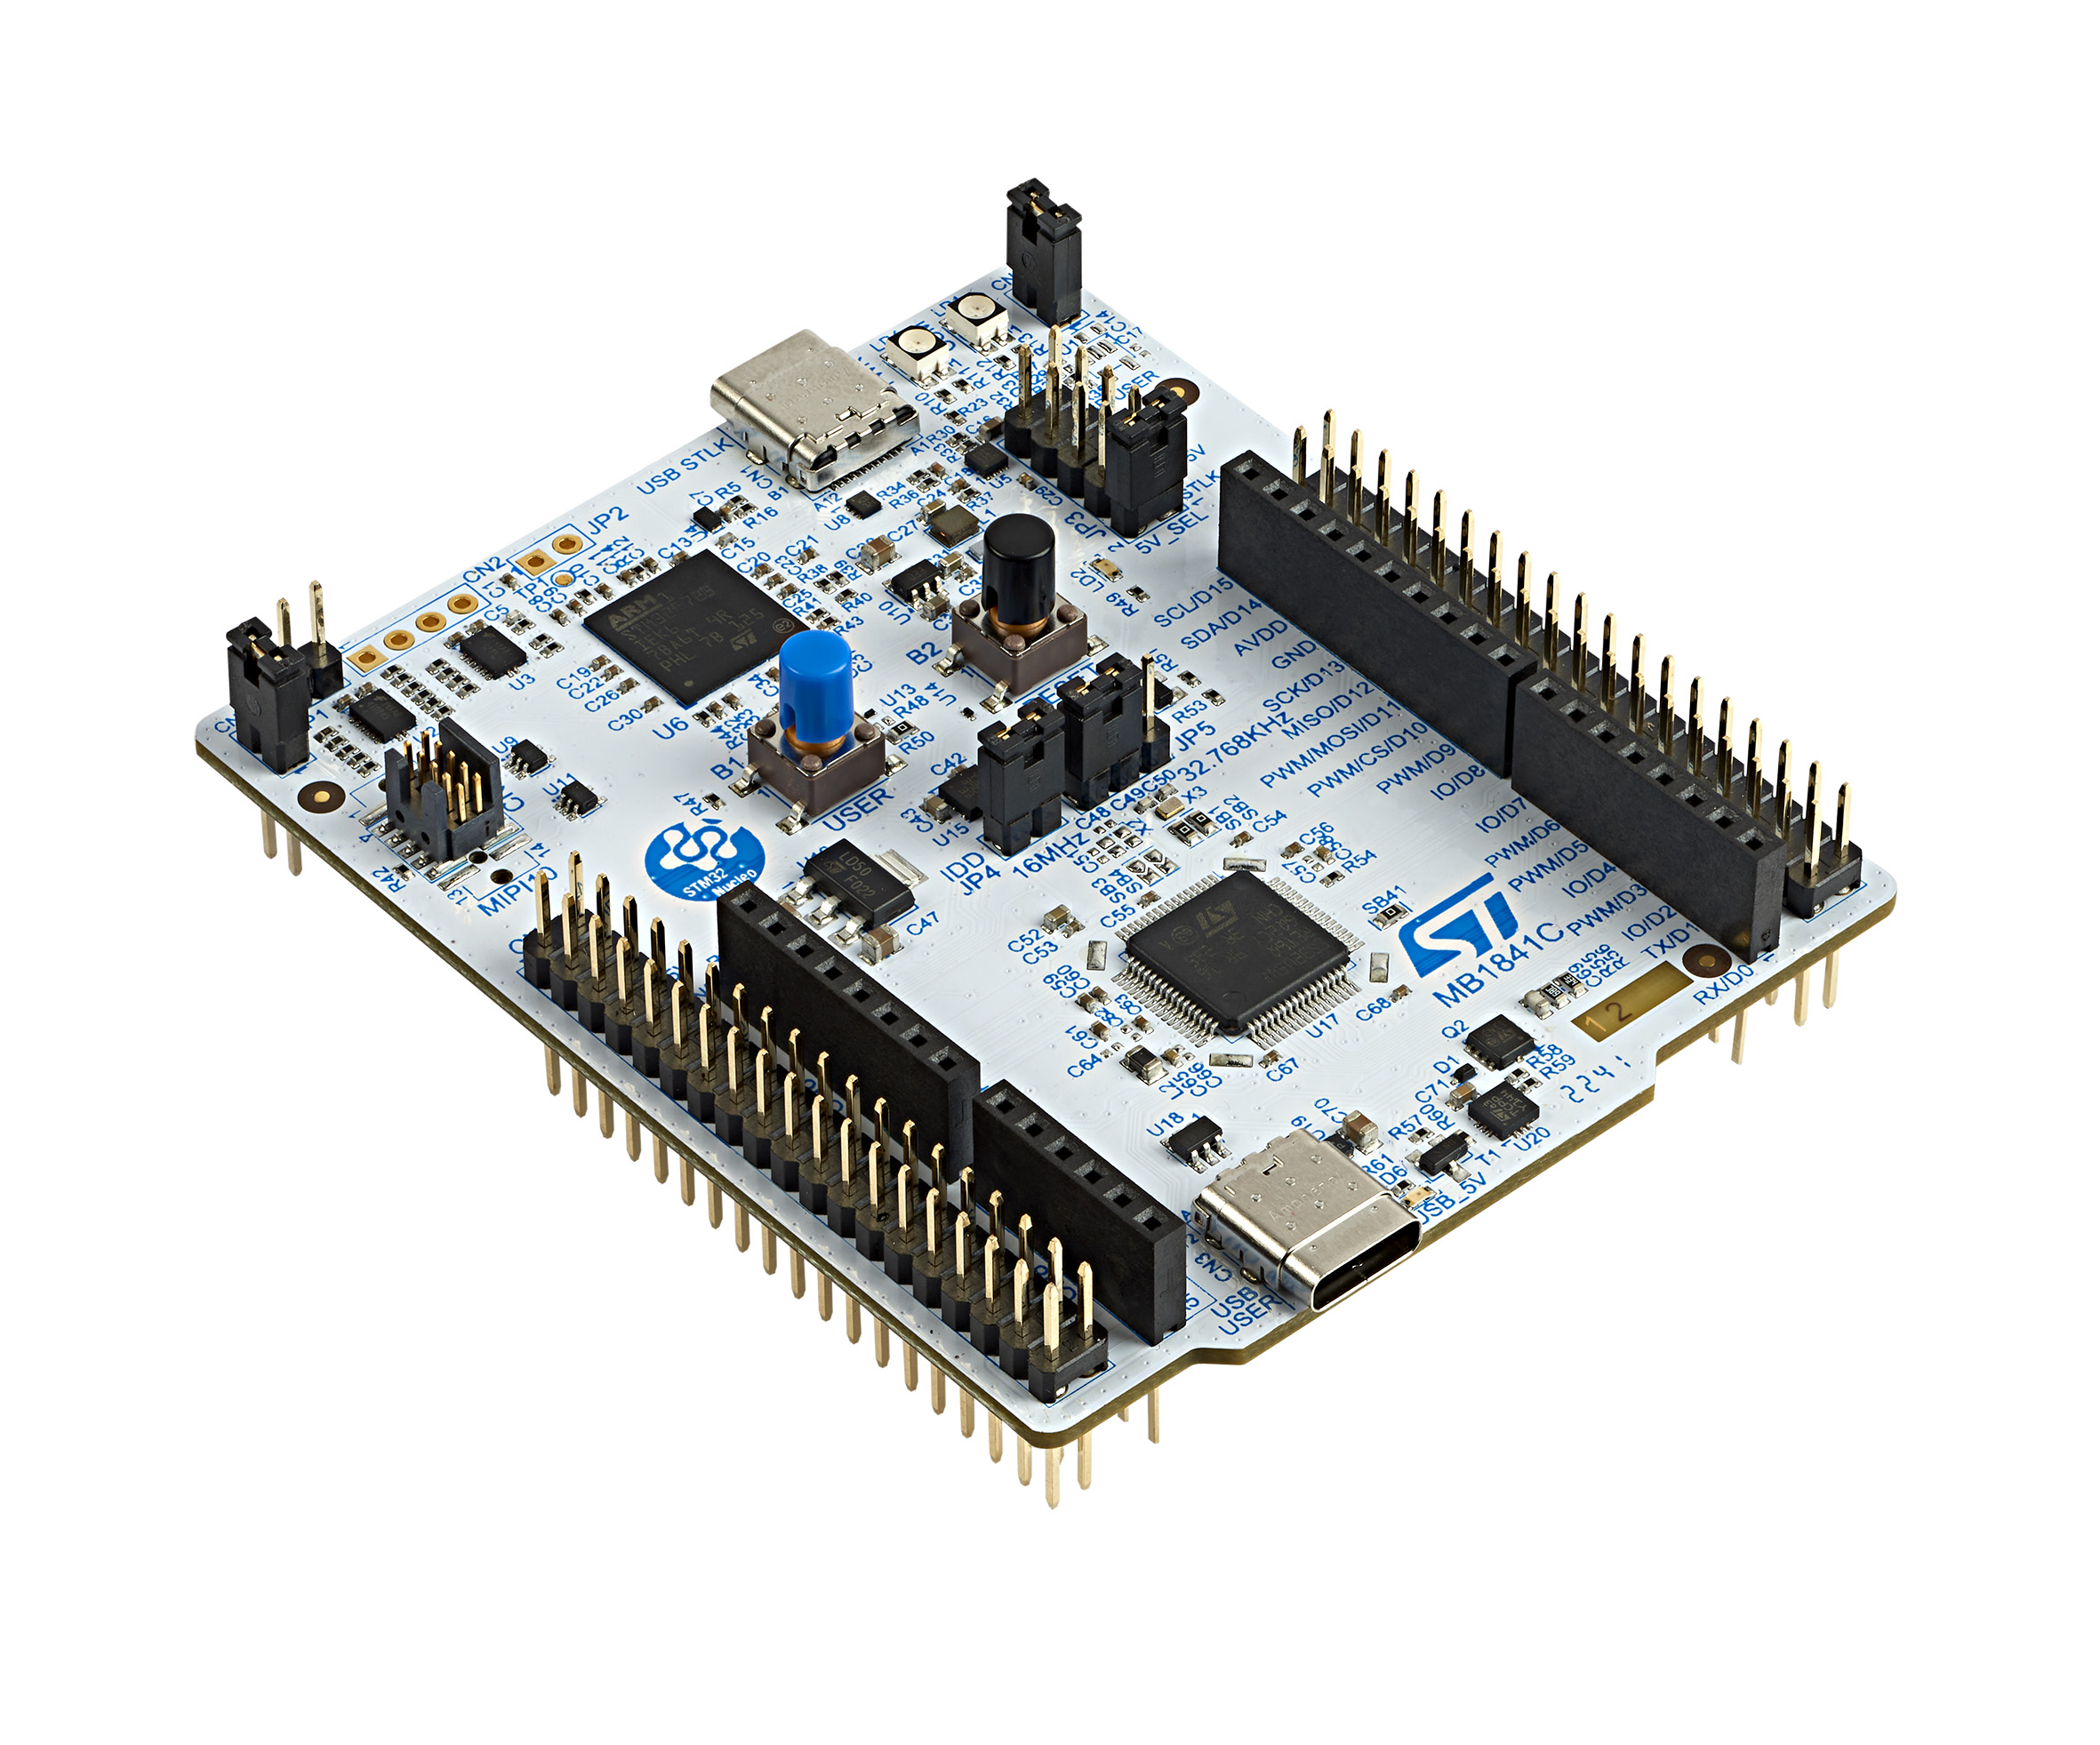
\includegraphics[width=6cm]{img/U5 Nucleo.jpg}
  \caption{STM32U545 Nucleo Board}
  \label{fig:stm32u545n}
\end{figure}
\end{itemize}

\subsection{Software Resources}
The following software tools were used for the  development, debugging and testing of the "CryptoEngine" demonstration:

\subsubsection{IAR Embedded Workbench}
IAR Embedded Workbench is an integrated development environment (IDE) used for programming, debugging, and optimizing embedded applications. It provides comprehensive support for STM32 microcontrollers, including the STM32XX and STM32U5 series. Key features include:
\begin{itemize}
    \item Advanced debugging capabilities with breakpoints, watch windows, and real-time data visualization.
    \item Code optimization tools to improve performance and reduce memory footprint.
    \item Integrated support for STM32CubeMX, allowing seamless project setup and configuration.
\end{itemize}
\begin{figure}[H]
  \centering
  
\includegraphics[width=8cm]{img/IAR.png}
  \caption{IAR Embedded Workbench}
  \label{fig:IAR}
\end{figure}

\subsubsection{STM32CubeMX}
STM32CubeMX is a graphical software configuration tool that simplifies the development of STM32-based applications. It allows developers to:
\begin{itemize}
    \item Configure microcontroller peripherals and middleware components through an intuitive graphical interface.
    \item Generate initialization code for STM32 microcontrollers, reducing development time.
    \item Integrate with various IDEs, including IAR Embedded Workbench, for a streamlined development workflow.
\end{itemize}
\begin{figure}[H]
  \centering
  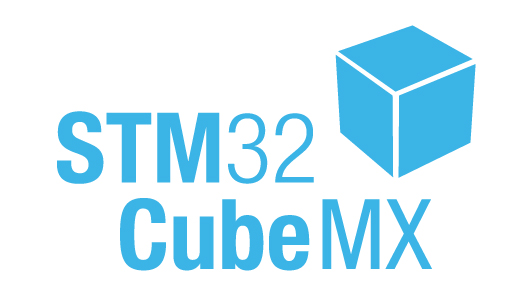
\includegraphics[width=8cm]{img/CUBEMX.jpg}
  \caption{STM32CubeMX}
  \label{fig:mx}
\end{figure}
\subsubsection{Yet Another Terminal (YAT)}
Yet Another Terminal (YAT) is a terminal application used for serial communication with the STM32 microcontrollers. It provides a user-friendly interface for monitoring and interacting with the microcontroller's output. Key features include:
\begin{itemize}
    \item Support for multiple communication protocols, including USART.
    \item Real-time data logging and visualization capabilities.
    \item Customizable settings for baud rate, data bits, parity, and stop bits.
\end{itemize}
\section*{Conclusion}
The work environment for this internship project includes both hardware and software resources that are essential for the successful implementation and demonstration of the "CryptoEngine" peripheral. The STM32XX MCU provides the necessary hardware capabilities, while the STM32U545 MCU is used for comparison and interoperability, utilizing AES and PKA peripherals. IAR Embedded Workbench and STM32CubeMX offer powerful tools for software development and configuration. Together, these resources enable the creation of a secure, efficient, and user-friendly cryptographic demonstration.
